\chapter{Programación de funciones combinacionales.}

\section{\obj}
\capacidad
\begin{itemize}
    \item  Programar funciones booleanas combinacionales en Arduino.
    \item  Verificar la compuertas NAND y NOR son en si mismas un conjunto Universal, equivalentes a el conjunto de conectivas lógicas OR, AND y NOT.
    \item Verificar que a partir de los mintérminos de una expresión lógica se obtienen los circuitos con compuertas NAND y de los maxtérminos, los circuitos con compuertas NOR.
    \item Verificar que para obtener la solución mínima de un circuito lógico, es necesario sintetizar los circuitos tanto por mintérminos como por maxtérminos. 
    \item Programar multiplexores $4\times1$ y $8\times1$.
    \item Programar un Decodificador Binario a Decimal.
\end{itemize} 


\section{\mat}
\begin{itemize}
    \item 1 Arduino UNO o equivalente: MEGA o ESP32.
    \item 1 Multímetro.
    \item 10 Resistencias de 270 o 330 $\Omega$.
    \item 5 Resistencias de 1k$\Omega$.
    \item 10 interruptores pulsadores.
    \item 1 Protoboard.
    \item 10 Diodes emisor de luz (LEDs).
    \item 1 Computadora portátil.
\end{itemize} 

\section{Marco de referencia}

Un circuito combinacional digital es un circuito que produce una o varias salidas en función de sus entradas actuales. Es decir, no mantiene ningún estado interno y su salida depende exclusivamente de sus entradas en el momento actual.
Existen muchas formas de implementar circuitos combinacionales, a partir de contactos eléctricos, válvulas neumáticas, transistores, software, etc. Sin embargo cualquier circuito lógico combinacional se puede expresar mediante cuatro formas equivalentes que describen su funcionamiento: ecuación lógica, tabla de verdad, diagrama de tiempo, y circuito eléctrico. 
Puede encontrar información adicional en el siguiente enlace \href{https://es.wikipedia.org/wiki/Sistema_combinacional}{https://es.wikipedia.org/wiki/Sistema\_combinacional}.   

\subsection{Implementan de expresiones Booleanas }

Un circuito combinacional  puede ser representado de distintas formas, pero la más común es mediante una ecuación lógica, por ejemplo: 
\begin{equation}
\label{Ec1}
F(a,b,c)=a\cdot b+\bar{a}\cdot \bar{b}\cdot c
\end{equation}

La expresión anterior posee una representación en suma de productos (SDP), puede ser implementada en C de la siguiente forma:

		 \begin{lstlisting}[language=Arduino,numbers=none, showstringspaces=false]
		bool F(bool a,bool b,bool c){
			return  (a && b) || (!a && !b && c);
		}
		\end{lstlisting} 

Existen ocho formas estándar de implementar la ecuación \eqref{Ec1} digital-mente y por consecuencia en software . Otras maneras de implementar las funciones lógicas  son con el producto de sumas (PDS), las implementaciones a dos niveles  NAND/NAND y NOR/NOR, todas las implementaciones deben arrojar los mismos resultados.

Por otra parte, la ecuación \eqref{Ec1} es equivalente a la expresión booleana  NAND/NAND si se niega dos veces y se aplica el \href{https://es.wikipedia.org/wiki/Leyes_de_De_Morgan}{Teorema de Morgan}.


\begin{align}
\label{Ec2}
F(a,b,c)&=a\cdot b+\bar{a}\cdot \bar{b} \cdot c \\
F(a,b,c)&=\overline{\overline{a\cdot b+\bar{a}\cdot \bar{b}\cdot c}} \\  \label{Ec3}
F(a,b,c)&=\overline{\overline{a\cdot b}\cdot\overline{\bar{a}\cdot \bar{b}\cdot c}}
\end{align}


Notece que la ecuacion \eqref{Ec3} necesita conectivas lógicas (funciones) de 2 y 3 entradas. Esto no es un problema cuando se implementa en SOFTWARE, pero sí se requiere hacer una implementación fisica hay que aplicar el Algebra Booleana para dejar la expresión en términos de conectivas de solamente dos entradas. Lo que se hace es que el término de tres literales, le aplicamos una doble negación tal como sigue.

\begin{eqnarray}
\label{Ec5}
F(a,b,c)=\overline{\overline{a\cdot b}\cdot\overline{\overline{\overline{\bar{a}\cdot \bar{b}}}\cdot c}} 
\end{eqnarray}

La expresión \eqref{Ec5} se encuentra en términos de conectivas NAND de dos entradas y se puede implementar en ARDUINO  de la siguiente forma:
{\footnotesize 
\begin{lstlisting}[language=Arduino,numbers=none, showstringspaces=false]
bool F(bool a, bool b, bool c){
	bool result = false;
	result = NAND(NAND(a,b),NAND(NAND(NAND(NAND(a,true),NAND(b,true)),true),c));
	return result;
}
\end{lstlisting} 
}
donde la NAND de dos entradas es:

		\begin{lstlisting}[language=Arduino,numbers=none, showstringspaces=false]
		bool NAND(bool x, bool y){
			return !(x && y);
		}
		\end{lstlisting}

\subsection{Multiplexores y Decodificadores}

Un \href{https://es.wikipedia.org/wiki/Multiplexor}{multiplexor} (Mux) es un circuito combinacional con $2^{n}$ entrada, más $n$  entradas selectoras o de control y una salida. Este circuito combinacional selecciona con las $n$ entradas control,  el valor booleano de una entrada entre $\left[ 0,2^{n}-1\right]$ y coloca dicho valor en la salida. La ecuación general de cualquier multiplexor es la siguiente,

\begin{equation}
MUX=\sum_{i=0}^{2^{n}-1} I_{i}\cdot \mathbb{S}_i
\end{equation}
donde $\mathbb{S}_i$  es la $i$-ésima permutacion de las entradas de selección. A modo de ejemplo un Mux $2 \times 1$
 posee dos entradas digitales, una de control y una salida. Un Mux $4 \times 1$ posee cuatro entradas digitales, dos de control y una salida, Un Mux $8 \times 1$ posee ocho entradas digitales, tres de control y una salida.
 
La ecuación de un Mux $4 \times 1$ es la siguiente,

\begin{equation}
	F(I_0,I_1,I_2,I_3,S_1,S_0)=I_0\bar{S_1}\bar{S_0}+I_1\bar{S_1}S_0+I_2S_1\bar{S_0}+I_3S_1S_0
\end{equation} 

El código para implementar dicho multiplexor es similar al siguiente,
{\footnotesize 
\begin{lstlisting}[language=Arduino,numbers=none, showstringspaces=false]
bool F(bool I0,bool I1,bool I2,bool I3,bool S1,bool S0){
	return (I0&&!S1&&!S0 || I1&&!S1&&S0 || I2&&S1&&!S0 || I3&&S1&&S0) ;
}
\end{lstlisting}
}
Los circuitos que realizan función inversa del multiplexor se  llama \href{https://es.wikipedia.org/wiki/Demultiplexor}{Demultiplexores}  y usualmente tiene una entrada digital más $n$ entradas de selección y $2^{n}$ salidas digitales.

Otro ejemplo de circuito combinacional son los \href{URL}{Decodificadores} y \href{https://es.wikipedia.org/wiki/Codificador}{Codificadores}.  Un codificador es un circuito combinacional con $2^{n}$ entradas y $n$ salidas, cuya misión es presentar en la salida el código binario correspondiente a la entrada activada. Mientras que un decodificador hace el trabajo inverso, recibe un código binario y lo transforma en cualquier otro código, ya sea  binarios como el Gray o exceso 3; o otras reprentaciones numericas: octal, decimal, hexagecimal. La figura \ref{fig:decoderexample} muestra la implementan digital de un decodificador de 2 a 4 líneas, la tabla de verdad del circuito y las ecuaciones características de cada salida. 
\begin{figure}
	\centering
	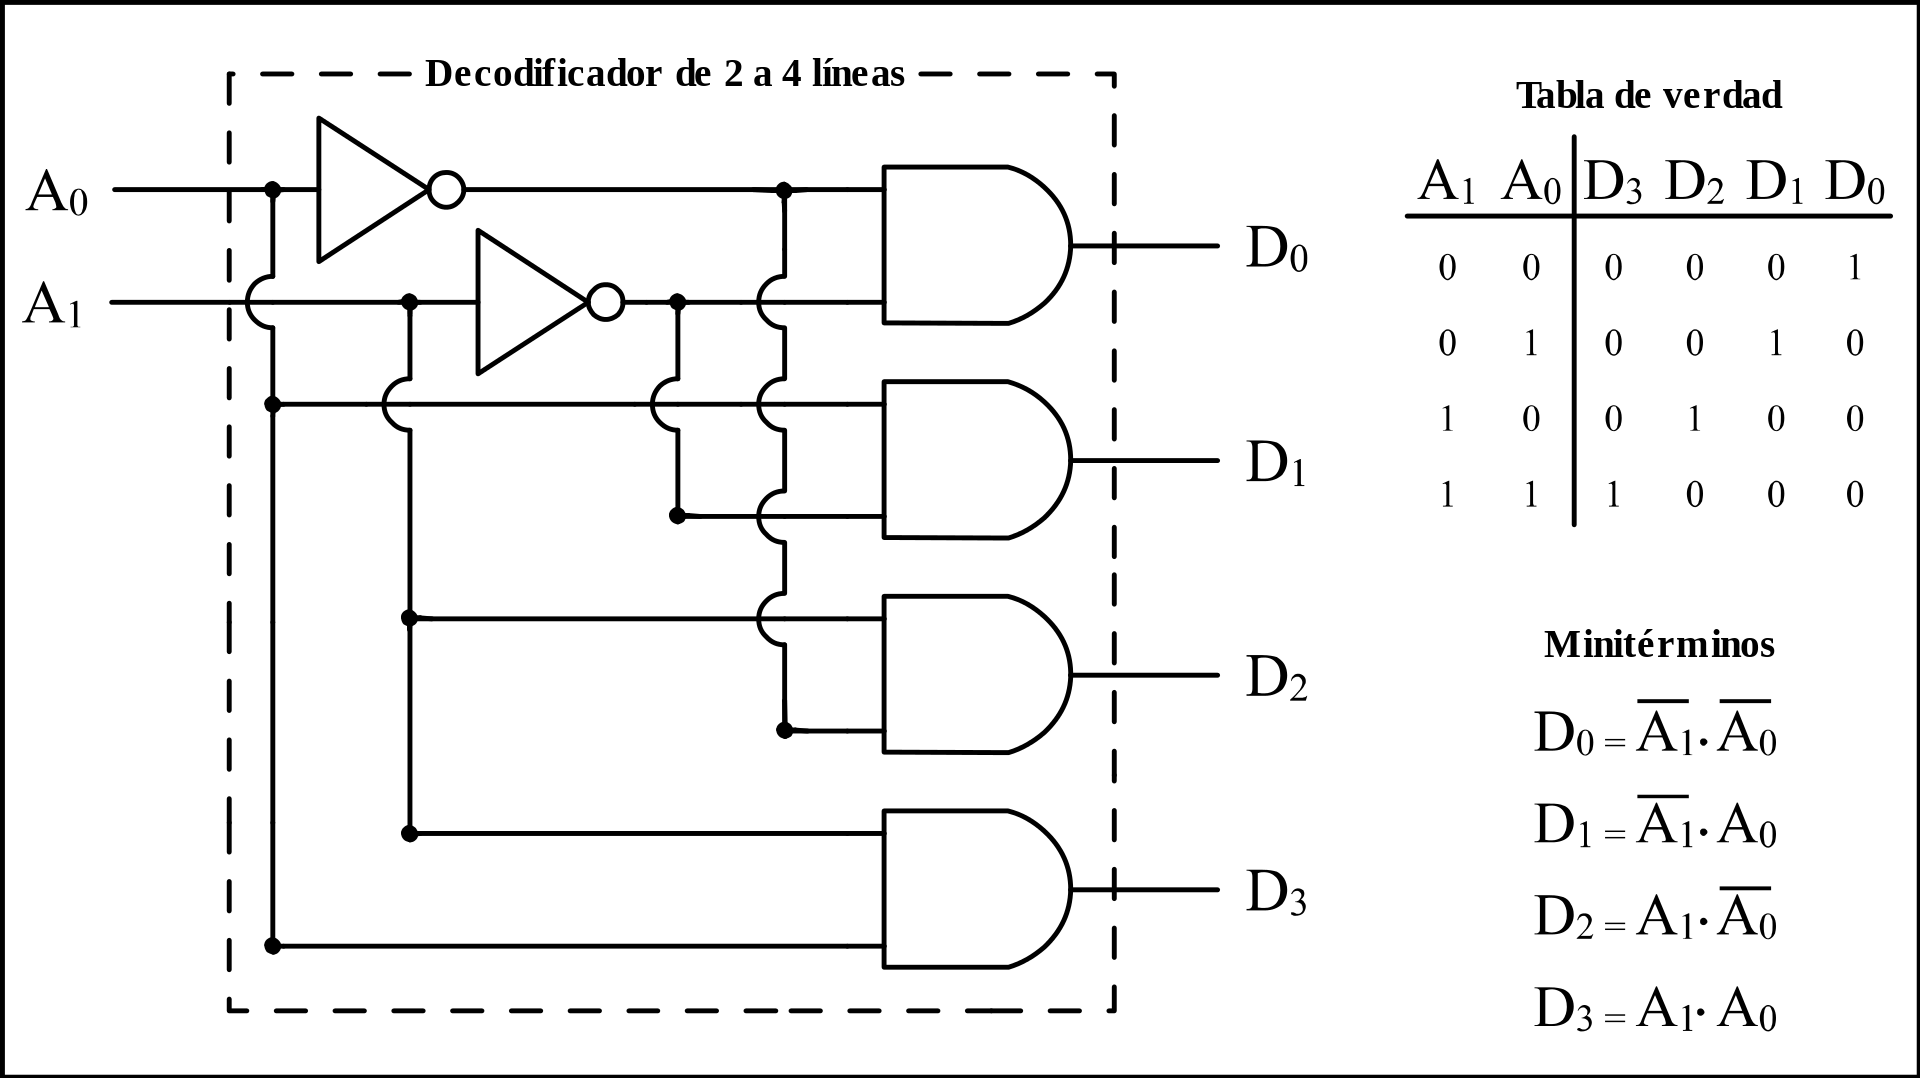
\includegraphics[width=0.7\linewidth]{fig/Decoder_Example.png}
	\caption{Decodificador de código binario de dos bits a cuatro líneas de salida.  }
	\label{fig:decoderexample}
\end{figure}

Una posible implementación para Arduino de este decodificador es la siguiente.

\begin{lstlisting}[language=Arduino,numbers=none, showstringspaces=false]
	byte  DECO (bool A0, bool A1)
	{
		int i=0;
		bool D[4]={false, false, false, false};
		byte deco=0;
	
		D[0]=!A1 && !A0;
		D[1]=!A1 && A0;
		D[2]=A1 && !A0;
		D[3]=A1 && A0;
	
		for (i=0; i<sizeof(D);i++)
		{
			bitWrite(deco, i, D[i]);
		}
	return deco;
	}
\end{lstlisting}
  
\section{Metodología}

Este laboratorio tiene una duración de 4 lecciones, repartidas en dos semanas. Los estudiantes deben mostrar durante las clases programadas las tres actividades propuestas. Deben recabar fotografías y resultados de los equipos de medición para elaborar las evidencias. Las evidencias se subirán al TecDigital la semana siguiente finalizadas las actividades.

\section{Práctica en Clase}

\subsection{Actividad 1}

Programe en Arruino una lógica combinacional que resuelva el siguiente problema:
\begin{itemize}
    \item En una planta industrial se desea automatizar un motor y una alarma de acuerdo a 4 sensores llamados $a$, $b$, $c$ y $d$ 
    \item La señal del motor se representa por la función lógica $f1$, y se activará  cuando los sensores $a$ y $b$ estén encendidos, o cuando los sensores $b$ y $d$ estén encendidos, o cuando los sensores $a$, $c$ y $d$ están encendidos.
    \begin{equation*}
        f1 = ab + bd + acd
    \end{equation*}
    \item La señal de  alarma se representa con la función lógica $f2$, y se activará siempre que estén todos los sensores apagados excepto $a$ o todos apagados excepto $c$ o estén encendidos $c$ y $d$ y el resto apagados. También la alarma se enciende cuando todos los sensores están encendidos o cuando están todos encendidos excepto $d$ o todos encendidos excepto $c$.
    \begin{equation*}
        f2 = a\bar{b}\bar{c}\bar{d} + \bar{a}\bar{b}c\bar{d} + \bar{a}\bar{b}cd + abcd + abc\bar{d} + ab\bar{c}d
    \end{equation*}
    \begin{equation*}
        f2 = a\bar{b}\bar{c}\bar{d} + \bar{a}\bar{b}c + abc + abd
    \end{equation*}
    \item Los pines $\left\lbrace 2,3,4,5\right\rbrace$ serán las entradas digitales $\left\lbrace a,b,c,d\right\rbrace$.
    \item Los pines $\left\lbrace 6,7,8\right\rbrace $ se reservan para $f1$. Se deben implementar tres funciones: la suma de productos $(SDP)$, el producto de sumas $(PDS)$ y la función resuelta por conectivas $NAND/NAND$. 
    \item Los pines $\left\lbrace 8,9,10\right\rbrace $ se reservan para $f2$. Se deben implementar tres funciones: la suma de productos $(SDP)$, el producto de sumas $(PDS)$ y la función resuelta por conectivas $NOR/NOR$.
\end{itemize}
 
\subsubsection{Conteste las preguntas:}

¿Cómo sería el circuito digital de cada una de las funciones implementadas?
¿Como es la tabla de verdad experimental de cada salida versus la tabla teórica?


\subsection{Actividad 2}

Programe las funciones de un Multiplexor 2x1, 4x1 y 8x1.
Por otra parte, existe un circuito  combinacional que se comporta como la tabla de verdad mostrada en la Tabla \ref{tab:tv}.

\begin{table}[H]
\centering
\caption{Comportamiento esperado de la estructura lógica.}
\label{tab:tv}
\begin{tabular}{ccc}
    \toprule 
    $a$ & $b$ & $F(a,b)$ \\ 
    \midrule
    0 & 0 & $c + d$ \\ 
    0 & 1 & $\overline{c + d}$ \\ 
    1 & 0 & $\overline{c \cdot d}$ \\ 
    1 & 1 & $c \oplus d$ \\ 
    \bottomrule
\end{tabular} 

\end{table}

\subsubsection{Conteste las preguntas:}

¿El comportamiento de un multiplicador $8 \times 1$ coincide con la tabla teórica?
En la funcion Loop() , llame la función del MUX  $8 \times 1$ e ingrese parámetros $\left\lbrace a,b,c,d \right\rbrace $ de tal forma que se comporte igual que la tabla de verdad presentada en el Cuadro \ref{tab:tv}.¿Tiene el mismo comportamiento?
¿Es posible implementar la T.V. con dos MUX $4 \time 1$ y un MUX  $2 \time 1$?¿Como se implementa?
